\section{Introduction}
Hardware performance counters are architecture-specific special-purpose registers integrated into modern central processing units (CPUs) used for performance profiling.
As an example, modern Intel processors support hardware counters that report events such as CPU utilization, L1 cache misses, branch mispredictions and a host of other CPU-specific performance indicators.
This information is invaluable when profiling low-level software performance.
What is more, compared to traditional software-based profiling, hardware performance counters incur negligible overhead because they are integrated into the hardware.
However, support for hardware counters is still in early stages, and was not integrated into the Linux kernel until the 2.6.31 release.
In addition, some architectures support hardware counters, but have a hard limit on the number of events, sometimes only two or four, that can be monitored at a time.

Tiptop~\cite{rohou:hal-00639173} is an application developed by Erven Rohou\footnote{\texttt{erven.rohou@inria.fr}} and is an attempt towards an intuitive interface for accessing hardware performance counters in modern CPUs.
The interface for tiptop is similar to the popular top\footnote{\texttt{\url{http://sourceforge.net/projects/unixtop/}}} utility. 
In tiptop's default configuration, it provides real-time per-process hardware counter statistics, such as the number of CPU instructions executed per-process.
The values that appear on the real-time screen are configurable by the user.
Through use of an XML file, multiple screens can be configured and flipped through.
In Figure~\ref{fig:tiptop-default} we have a screenshot of tiptop's default screen, and highlight a few of its key features.

Despite tiptop's advantages, we identified a number of limitations.
As one example, the Pentium III supports 80 hardware counter events, but can track at most two in parallel~\cite{hpc-trusted}.
However, the default tiptop screen assumes that the underlying architecture can track five hardware counters events.
In addition, we found that building XML files was cumbersome and platform-specific.
To compound this problem, tiptop exposes less than 20\% of the hardware performance counters available across platforms.
In many cases, tracking a hardware counter not currently supported by tiptop requires modification and recompilation of tiptop's C source files.

In light of these limitations, we identified two feature enhancements for tiptop.
First, we enhanced tiptop to display the number of threads per-process as a default feature.
Then, as a substantial feature enhancement, we integrated the cross-platform Performance Application Programming Interface (PAPI)~\cite{Mucci99papi:a} library into tiptop as an alternative API to access hardware counters. (This is backwards-compatible change, and use of the PAPI API is optional when creating an XML configuration file.)
Integration with PAPI increases the breadth of platforms and kernel versions supported by tiptop.
Now, tiptop can run with kernel versions prior to 2.6.31, via a PAPI-supplied kernel patch.
In addition, through software multiplexing, PAPI enables the number of hardware counter events to exceed the hard limit imposed by the hardware.
Finally, the integration with PAPI simplifies the process of creating cross-platform XML configuration files for tiptop hardware counters can be specified by using PAPI-specific macros, by abstracting architecture-specific configuration options from the user.

In addition to feature enhancements, we identified two tiptop bugs, and confirmed them through personal communications with lead developer Erven Rohou.
Both bugs prevent tiptop from correctly displaying hardware counter statistics under specific conditions.
For the first bug, we identified a solution that minimizes the probability that the bug occurs, and will work with Erven Rohou to include our patch into the main branch of the tiptop source.
The second bug remains unresolved, but can be avoided by running tiptop as root.

In section~\ref{sec:methodology} we give an overview of our high-level development cycle and the tools we used to repair and enhance tiptop.
In section~\ref{sec:results} we give further details about our feature enhancements and bugfixes.
We conclude in section~\ref{sec:conclusion} with a discussion about additional feature improvements for future versions of tiptop.

\begin{figure}[t]
\footnotesize
\centering
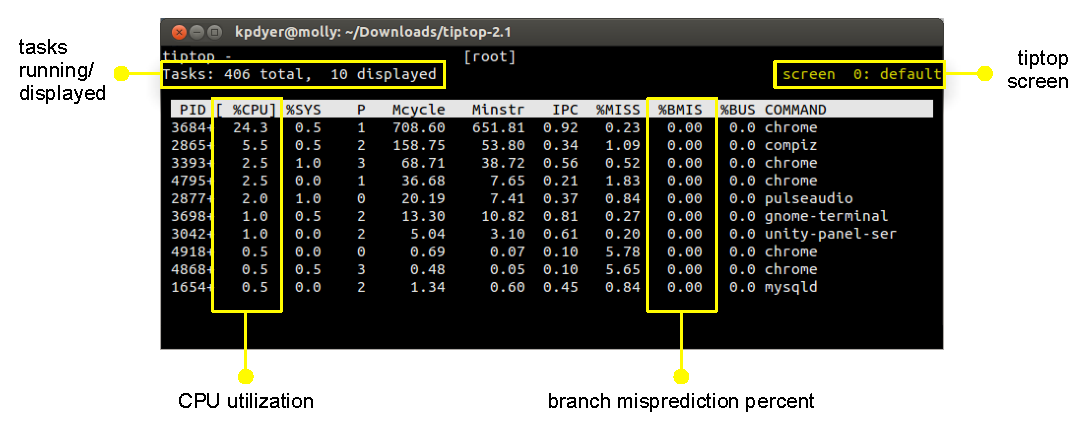
\includegraphics[width=1\textwidth]{tiptop-default}
%\hspace{.1in}
%\includegraphics[width=0.48\textwidth]{tiptop-default-screenshot-1}
\caption{A screenshot of the default screen for tiptop version 2.1. Each row in the display represents a single process.
In the top-left corner we have the number of running and displayed processes.
By default, tiptop only displays processes that have non-zero CPU utilization.
In the bottom-left we highlight the CPU utilization, reported as percentage of cycles used since the last screen refresh.
In the bottom-right corner we highlight the number of branch mispredictions.
Finally, in the top-right we highlight the label for the current screen.
Multiple views with custom columns can be configured and flipped through (using the right and left arrow keys) in real-time.}
\label{fig:tiptop-default}
\end{figure}